\documentclass[10pt,twoside]{article}

\newcommand{\reporttitle}{Mars Rover}
\newcommand{\reportauthor}{}
\newcommand{\reporttype}{Project Report}


% include files that load packages and define macros
%%%%%%%%%%%%%%%%%%%%%%%%%%%%%%%%%%%%%%%%%
% University Assignment Title Page 
% LaTeX Template
% Version 1.0 (27/12/12)
%
% This template has been downloaded from:
% http://www.LaTeXTemplates.com
%
% Original author:
% WikiBooks (http://en.wikibooks.org/wiki/LaTeX/Title_Creation)
%
% License:
% CC BY-NC-SA 3.0 (http://creativecommons.org/licenses/by-nc-sa/3.0/)
% 
% Instructions for using this template:
% This title page is capable of being compiled as is. This is not useful for 
% including it in another document. To do this, you have two options: 
%
% 1) Copy/paste everything between \begin{document} and \end{document} 
% starting at \begin{titlepage} and paste this into another LaTeX file where you 
% want your title page.
% OR
% 2) Remove everything outside the \begin{titlepage} and \end{titlepage} and 
% move this file to the same directory as the LaTeX file you wish to add it to. 
% Then add \input{./title_page_1.tex} to your LaTeX file where you want your
% title page.
%
%----------------------------------------------------------------------------------------
%	PACKAGES AND OTHER DOCUMENT CONFIGURATIONS
%----------------------------------------------------------------------------------------
\usepackage{ifxetex}
\usepackage{textpos}
\usepackage[numbers]{natbib}
\usepackage{kpfonts}
\usepackage[a4paper,hmargin=1.5cm,vmargin=1.5cm,includeheadfoot]{geometry}
\usepackage{ifxetex}
\usepackage{stackengine}
\usepackage{tabularx,longtable,multirow,subfigure,caption}%hangcaption
\usepackage{fncylab} %formatting of labels
\usepackage{fancyhdr}
\usepackage{color}
\usepackage[tight,ugly]{units}
\usepackage{url}
\usepackage{float}
\usepackage[english]{babel}
\usepackage{amsmath}
\usepackage{graphicx}
\usepackage[colorinlistoftodos]{todonotes}
\usepackage{dsfont}
\usepackage{epstopdf} % automatically replace .eps with .pdf in graphics
\usepackage{backref}
\usepackage{array}
\usepackage{latexsym}
\usepackage{etoolbox}
\usepackage{tikz}
\usepackage{multirow}
\usepackage{booktabs}
\usepackage[toc,page]{appendix}
\usepackage{listings}
\usepackage{xfrac}
\usepackage{titlesec}
%\usepackage{enumerate} % for numbering with [a)] format 
\setlength{\parskip}{1em}

%%%%%%%%%% SAM VERILOG %%%%%%%%%%%%%%%%%%%%%%

\usepackage{minted}
\usemintedstyle{manni}  %manni

%%%%%%%%%%%%%%%%%%%%%%%%%%%%%%%%%%%%%%%%%%%%%%

\ifxetex
\usepackage{fontspec}
\setmainfont[Scale=.8]{OpenDyslexic-Regular}
\else
\usepackage[pdftex,pagebackref,hypertexnames=false,colorlinks]{hyperref} % provide links in pdf
\hypersetup{pdftitle={},
  pdfsubject={}, 
  pdfauthor={\reportauthor},
  pdfkeywords={}, 
  pdfstartview=FitH,
  pdfpagemode={UseOutlines},% None, FullScreen, UseOutlines
  bookmarksnumbered=true, bookmarksopen=true, colorlinks,
    citecolor=black,%
    filecolor=black,%
    linkcolor=black,%
    urlcolor=black}
\usepackage[all]{hypcap}
\fi

\usepackage{tcolorbox}

% various theorems
\usepackage{ntheorem}
\theoremstyle{break}
\newtheorem{lemma}{Lemma}
\newtheorem{theorem}{Theorem}
\newtheorem{remark}{Remark}
\newtheorem{definition}{Definition}
\newtheorem{proof}{Proof}

% example-environment
\newenvironment{example}[1][]
{ 
\vspace{4mm}
\noindent\makebox[\linewidth]{\rule{\hsize}{1.5pt}}
\textbf{Example #1}\\
}
{ 
\noindent\newline\makebox[\linewidth]{\rule{\hsize}{1.0pt}}
}



%\renewcommand{\rmdefault}{pplx} % Palatino
% \renewcommand{\rmdefault}{put} % Utopia

\ifxetex
\else
\renewcommand*{\rmdefault}{bch} % Charter
\renewcommand*{\ttdefault}{cmtt} % Computer Modern Typewriter
%\renewcommand*{\rmdefault}{phv} % Helvetica
%\renewcommand*{\rmdefault}{iwona} % Avant Garde
\fi

\setlength{\parindent}{0em}  % indentation of paragraph

\setlength{\headheight}{14.5pt}
\pagestyle{fancy}
\fancyfoot[ER,OL]{\thepage}%Page no. in the left on
                                %odd pages and on right on even pages
\fancyfoot[OC,EC]{\sffamily }
\renewcommand{\headrulewidth}{0.1pt}
\renewcommand{\footrulewidth}{0.1pt}
\captionsetup{margin=10pt,font=small,labelfont=bf}


%--- chapter heading

\def\@makechapterhead#1{%
  \vspace*{10\p@}%
  {\parindent \z@ \raggedright %\sffamily
        %{\Large \MakeUppercase{\@chapapp} \space \thechapter}
        %\\
        %\hrulefill
        %\par\nobreak
        %\vskip 10\p@
    \interlinepenalty\@M
    \Huge \bfseries 
    \thechapter \space\space #1\par\nobreak
    \vskip 30\p@
  }}

%---chapter heading for \chapter*  
\def\@makeschapterhead#1{%
  \vspace*{10\p@}%
  {\parindent \z@ \raggedright
    \sffamily
    \interlinepenalty\@M
    \Huge \bfseries  
    #1\par\nobreak
    \vskip 30\p@
  }}
  



% %%%%%%%%%%%%% boxit
\def\Beginboxit
   {\par
    \vbox\bgroup
	   \hrule
	   \hbox\bgroup
		  \vrule \kern1.2pt %
		  \vbox\bgroup\kern1.2pt
   }

\def\Endboxit{%
			      \kern1.2pt
		       \egroup
		  \kern1.2pt\vrule
		\egroup
	   \hrule
	 \egroup
   }	

\newenvironment{boxit}{\Beginboxit}{\Endboxit}
\newenvironment{boxit*}{\Beginboxit\hbox to\hsize{}}{\Endboxit}



\allowdisplaybreaks

\makeatletter
\newcounter{elimination@steps}
\newcolumntype{R}[1]{>{\raggedleft\arraybackslash$}p{#1}<{$}}
\def\elimination@num@rights{}
\def\elimination@num@variables{}
\def\elimination@col@width{}
\newenvironment{elimination}[4][0]
{
    \setcounter{elimination@steps}{0}
    \def\elimination@num@rights{#1}
    \def\elimination@num@variables{#2}
    \def\elimination@col@width{#3}
    \renewcommand{\arraystretch}{#4}
    \start@align\@ne\st@rredtrue\m@ne
}
{
    \endalign
    \ignorespacesafterend
}
\newcommand{\eliminationstep}[2]
{
    \ifnum\value{elimination@steps}>0\leadsto\quad\fi
    \left[
        \ifnum\elimination@num@rights>0
            \begin{array}
            {@{}*{\elimination@num@variables}{R{\elimination@col@width}}
            |@{}*{\elimination@num@rights}{R{\elimination@col@width}}}
        \else
            \begin{array}
            {@{}*{\elimination@num@variables}{R{\elimination@col@width}}}
        \fi
            #1
        \end{array}
    \right]
    & 
    \begin{array}{l}
        #2
    \end{array}
    &%                                    moved second & here
    \addtocounter{elimination@steps}{1}
}
\makeatother

%% Fast macro for column vectors
\makeatletter  
\def\colvec#1{\expandafter\colvec@i#1,,,,,,,,,\@nil}
\def\colvec@i#1,#2,#3,#4,#5,#6,#7,#8,#9\@nil{% 
  \ifx$#2$ \begin{bmatrix}#1\end{bmatrix} \else
    \ifx$#3$ \begin{bmatrix}#1\\#2\end{bmatrix} \else
      \ifx$#4$ \begin{bmatrix}#1\\#2\\#3\end{bmatrix}\else
        \ifx$#5$ \begin{bmatrix}#1\\#2\\#3\\#4\end{bmatrix}\else
          \ifx$#6$ \begin{bmatrix}#1\\#2\\#3\\#4\\#5\end{bmatrix}\else
            \ifx$#7$ \begin{bmatrix}#1\\#2\\#3\\#4\\#5\\#6\end{bmatrix}\else
              \ifx$#8$ \begin{bmatrix}#1\\#2\\#3\\#4\\#5\\#6\\#7\end{bmatrix}\else
                 \PackageError{Column Vector}{The vector you tried to write is too big, use bmatrix instead}{Try using the bmatrix environment}
              \fi
            \fi
          \fi
        \fi
      \fi
    \fi
  \fi 
}  
\makeatother

\robustify{\colvec}

%%% Local Variables: 
%%% mode: latex
%%% TeX-master: "notes"
%%% End: 
 % various packages needed for maths etc.
% quick way of adding a figure
\newcommand{\fig}[3]{
 \begin{center}
 \scalebox{#3}{\includegraphics[#2]{#1}}
 \end{center}
}

%\newcommand*{\point}[1]{\vec{\mkern0mu#1}}
\newcommand{\ci}[0]{\perp\!\!\!\!\!\perp} % conditional independence
\newcommand{\point}[1]{{#1}} % points 
\renewcommand{\vec}[1]{{\boldsymbol{{#1}}}} % vector
\newcommand{\mat}[1]{{\boldsymbol{{#1}}}} % matrix
\newcommand{\R}[0]{\mathds{R}} % real numbers
\newcommand{\Z}[0]{\mathds{Z}} % integers
\newcommand{\N}[0]{\mathds{N}} % natural numbers
\newcommand{\nat}[0]{\mathds{N}} % natural numbers
\newcommand{\Q}[0]{\mathds{Q}} % rational numbers
\ifxetex
\newcommand{\C}[0]{\mathds{C}} % complex numbers
\else
\newcommand{\C}[0]{\mathds{C}} % complex numbers
\fi
\newcommand{\tr}[0]{\text{tr}} % trace
\renewcommand{\d}[0]{\mathrm{d}} % total derivative
\newcommand{\inv}{^{-1}} % inverse
\newcommand{\id}{\mathrm{id}} % identity mapping
\renewcommand{\dim}{\mathrm{dim}} % dimension
\newcommand{\rank}[0]{\mathrm{rk}} % rank
\newcommand{\determ}[1]{\mathrm{det}(#1)} % determinant
\newcommand{\scp}[2]{\langle #1 , #2 \rangle}
\newcommand{\kernel}[0]{\mathrm{ker}} % kernel/nullspace
\newcommand{\img}[0]{\mathrm{Im}} % image
\newcommand{\idx}[1]{{(#1)}}
\DeclareMathOperator*{\diag}{diag}
\newcommand{\E}{\mathds{E}} % expectation
\newcommand{\var}{\mathds{V}} % variance
\newcommand{\gauss}[2]{\mathcal{N}\big(#1,\,#2\big)} % gaussian distribution N(.,.)
\newcommand{\gaussx}[3]{\mathcal{N}\big(#1\,|\,#2,\,#3\big)} % gaussian distribution N(.|.,.)
\newcommand{\gaussBig}[2]{\mathcal{N}\left(#1,\,#2\right)} % see above, but with brackets that adjust to the height of the arguments
\newcommand{\gaussxBig}[3]{\mathcal{N}\left(#1\,|\,#2,\,#3\right)} % see above, but with brackets that adjust to the height of the arguments
\DeclareMathOperator{\cov}{Cov} % covariance (matrix) 
\ifxetex
\renewcommand{\T}[0]{^\top} % transpose
\else
\newcommand{\T}[0]{^\top}
\fi
% matrix determinant
\newcommand{\matdet}[1]{
\left|
\begin{matrix}
#1
\end{matrix}
\right|
}



%%% various color definitions
\definecolor{darkgreen}{rgb}{0,0.6,0}

\newcommand{\blue}[1]{{\color{blue}#1}}
\newcommand{\red}[1]{{\color{red}#1}}
\newcommand{\green}[1]{{\color{darkgreen}#1}}
\newcommand{\orange}[1]{{\color{orange}#1}}
\newcommand{\magenta}[1]{{\color{magenta}#1}}
\newcommand{\cyan}[1]{{\color{cyan}#1}}


% redefine emph
\renewcommand{\emph}[1]{\blue{\bf{#1}}}

% place a colored box around a character
\gdef\colchar#1#2{%
  \tikz[baseline]{%
  \node[anchor=base,inner sep=2pt,outer sep=0pt,fill = #2!20] {#1};
    }%
}%
 % short-hand notation and macros
\setcounter{tocdepth}{2}    % Makes contents smaller
\graphicspath{ {figures/} }

\begin{document}

% Last modification: 2016-09-29 (Marc Deisenroth)
\begin{titlepage}

\newcommand{\HRule}{\rule{\linewidth}{0.5mm}} % Defines a new command for the horizontal lines, change thickness here


%----------------------------------------------------------------------------------------
%	LOGO SECTION
%----------------------------------------------------------------------------------------


    \begin{tikzpicture}[remember picture,overlay]
    \node[anchor=north west,inner sep=1cm] at (current page.north west)
          {
\includegraphics[width = 4cm]{./figures/imperial}\\[0.5cm] };
    \end{tikzpicture}


\begin{center} % Center remainder of the page

%----------------------------------------------------------------------------------------
%	HEADING SECTIONS
%----------------------------------------------------------------------------------------
\textsc{\LARGE \reporttype}\\[1.5cm] 
\textsc{\Large Imperial College London}\\[0.5cm] 
\textsc{\large Department of Electrical and Electronic Engineering}\\[0.5cm] 
%----------------------------------------------------------------------------------------
%	TITLE SECTION
%----------------------------------------------------------------------------------------

\HRule \\[0.4cm]
{ \huge \bfseries \reporttitle}\\ % Title of your document
\HRule \\[1.5cm]
\end{center}
%----------------------------------------------------------------------------------------
%	AUTHOR SECTION
%----------------------------------------------------------------------------------------

%\begin{minipage}{0.4\hsize}
\begin{center}
\textbf{Authors:}\\
Sam Taylor - 01705109\\
Martin Prusa - 01713176\\
Leonardo Garofalo - 01746454\\
Katherine Zhang - 01504365\\
Maximus Wickham - 01717673\\
Matilde Piccoli - 01764158 \\
\end{center}
\vspace{2cm}
\makeatletter
\centering
Date: \@date 

\vfill % Fill the rest of the page with whitespace



\makeatother


\end{titlepage}



\newpage

\tableofcontents

\newpage
\section{Abstract}
\section{Project Management}
\subsection{Project Structure}
The given timeline for the project was 5 weeks. The first week was allocated for research and planning. Each member carried out research on their own module and a meeting was held to identify the main tasks and create a tentative project timeline. From the second week on-wards, bi-weekly meetings were held: one meeting at the beginning of the week to set the targets for that week and one meeting in the middle of the week to check up on progress. Week 2 was planned to work on the basic functionalities for each module so that a very basic prototype of the rover could be put together. In week 3, more sophisticated implementations and additional functions were added. By the end of week 4, the design of each module was finalised and integration of the whole rover was completed. The final week of the project was used to clean up any issues with the integrated rover and make final adjustments. 

\subsection{Meeting Structure}
At the beginning of each week we held a 45 minute meeting. Each member would take 5 minutes to update the group on their progress on the targets set for the previous week, discuss any issues they found and set new targets for the week. Midway through the week we had a brief 20 minute meeting to check in on everyone’s progress and give the opportunity for the members to bring up any problems or difficulties they might have ran into and adjust plans accordingly.

\subsection{Tools Used for Project Management}
A Gantt chart was used to illustrate the main tasks to be completed for each module and set deadlines for their completion. It served as an effective method for tracking progress and keeping on track. 




The productivity software Notion was also used for each member to make notes of their initial design process, development and testing. It provided an easy method to share progress with the rest of the team. The shared calendar was used to set dates of meetings and mark internal deadlines. 
Git was used for version control.
\newpage
\section{Design Process}
\subsection{Structural and Functional Design}
\subsection{Problem Definition and Design Criteria}

\subsubsection{Drive}

\subsubsection{Energy}
The energy subsystem can be split into 4 top level sections which all combine to provide battery power and charging to the rover. These can then be broken down into smaller subsections which are more manageable and easier to test individually (Table \ref{tab:EnergySpec}). This also allows for more unique features to be added later on in the process. 

The Cell safety is the most important part of this subsystem as excessive charging/discharging can severely damage the LiFePO (Lithium Iron Phosphate) cells used in this project. This would not only hamper the longevity of the mars rover but could also lead to it's destruction. Hence a series configuration for the cells was decided upon to give the user more control over the current output/input. Cell balancing will therefore be key in keeping the cells SOH as consistent as possible.

It was decided that two cells will be sufficient in the design as this would open up a variety of possible configurations with the PV panels and SMPS power supplies. Even so, the programming and hardware ought to be easily scalable should another cell be needed for longer rover missions. This will be reflected in the Design Overview section where various options have been explored. 
  
\begin{table}[htp]
\renewcommand{\arraystretch}{1.3}
 \centering
\begin{tabular}{@{}cll@{}}
\toprule
\multicolumn{1}{l}{Section}                       & Criteria          & Description \\ \midrule
\multirow{8}{*}{Arduino}                          & Data Collection   & \parbox{0.61\linewidth}{The current and voltage should be recorded continuously for safety features}            \\
                                                  & Charge Strategy   & \parbox{0.61\linewidth}{Try to get near maximum possible capacity out of cells}            \\
                                                  & SOC Estimation    &  \parbox{0.61\linewidth}{Real time percentage capacity of the battery via coulomb counting}           \\
                                                  & SOH Maintenance   &  \parbox{0.61\linewidth}{Provide balancing of the cells and an estimation of the SOH}           \\
                                                  & PV MPPT algorithm &  \parbox{0.61\linewidth}{Get the maximum amount of power out of the PV Panels}           \\
                                                  & Communication     & \parbox{0.61\linewidth}{Transmit and receive data from Control}            \\
                                                  & Cell Safety    & \parbox{0.61\linewidth}{$I_{In}^{Max} = 250mA$, $I_{Out}^{Max} = 500mA$, $V_{Bat}^{Max} = 3.7V$, $V_{Bat}^{Min} = 2.3V$}            \\
                                                  & Rover Range     & 
                                                  \parbox{0.61\linewidth}{Work out Rover range from Drive current and speed} \\\midrule
\multicolumn{1}{l}{{\multirow{3}{*}{SMPS}}}       & Charging Buck/Boost        & \parbox{0.61\linewidth}{PV voltage                                                         stepped down to battery voltage}            \\
                                                  & Discharging Buck/Boost    & \parbox{0.61\linewidth}{Battery voltage stepped down to motor control voltage} \\ 
                                                  & Drive Current Required &
                                                  \parbox{0.61\linewidth}{$I_{Drive}^{Max}$ = 550mA} \\ \midrule
\multicolumn{1}{l}{\multirow{2}{*}{Battery Pack}} & Number of Cells   &  \parbox{0.61\linewidth}{2}           \\
\multicolumn{1}{l}{}                              & Configuration     & \parbox{0.61\linewidth}{Series to allow to better current limitation}            \\ \midrule
\multicolumn{1}{l}{{\multirow{3}{*}{PV Panels}}}                     & Configuration     &  \parbox{0.61\linewidth}{2x2 (Two in series then in parallel)}           \\ 
                                                  & Usage &
                                                  \parbox{0.61\linewidth}{A charging station setup in a sunlit area} \\ \bottomrule
\end{tabular}
\caption{\label{tab:EnergySpec} Energy Specification}
\end{table}

 

\newpage


\subsubsection{Vision}
The function of the vision system was broken into three general objectives of which the team agreed the vision system should achieve (See objectives below) .We agreed aspects like rover position and path finding would be better tackled by different subsystems. The following diagram shows the three main functions of Vision.

\begin{figure}[hbt!]
    \centering
    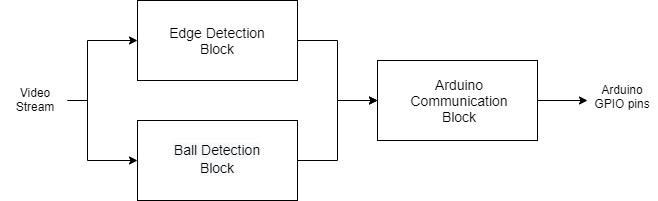
\includegraphics[scale=0.35]{HighLevelDesign.jpg}
    \captionsetup{justification=centering}
    \caption{High Level Block diagram}
\end{figure}

\smallbreak
After this high-level design i broke down each High level objective into a series of smaller objectives with several criteria which the subsystem would have to be meet to successfully accomplish its highlevel functionality. 
\smallbreak
\textbf{Ball detection:}

The diagram outlines a basic strategy for approaching the detection of balls through a process of highlighting , filtering and calculating. Each  ball occupies its own spectrum of colours in varying brightness conditions this spectrum can be highlighted so that we determine the maximum and minimum pixels of balls.Each block was designed to be testable by certain criteria so its success can be verified to ensure the entire block is functioning. 

\textbf{Edge detection:}

Calculating the luminance space of the image we can observe the brightness of each pixel which after the
application of a Sobel filter can be used to produce the edge space. This edge space can then be highlighted
using a threshold this highlighted space will reveal edges. .Each block was designed to be testable by certain
criteria so its success can be verified to ensure the entire block is functioning.

\textbf{Communication:}

This block facilitates communication between the Arduino ESP connected to the FPGA pins.It will utilise an agreed method to transfer data one way to the Control subsystem. All variables calculated in the analysis of the vision data will be relayed to it.


\begin{figure}[!htb]
    \centering
    \begin{minipage}{.33\textwidth}
        \centering
        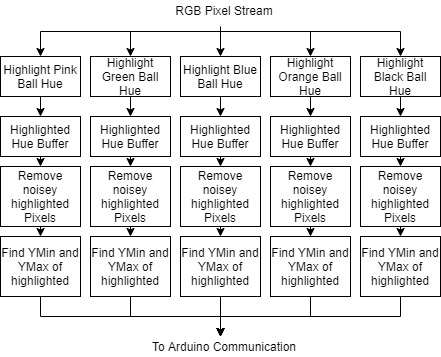
\includegraphics[width=0.8\linewidth, height=0.2\textheight]{BallDetection.jpg}
        \caption{Ball detection overview}
        \label{fig:BallDetectionOverview}
    \end{minipage}%
    \begin{minipage}{0.33\textwidth}
        \centering
        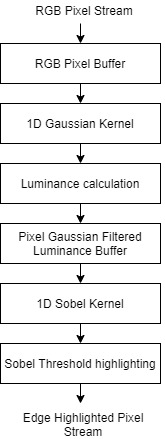
\includegraphics[width=0.4\linewidth, height=0.25\textheight]{EdgeDetection.jpg}
        \caption{Edge detection overview}
        \label{fig:EdgeDetectionOverview}
    \end{minipage}%
    \begin{minipage}{.33\textwidth}
        \centering
        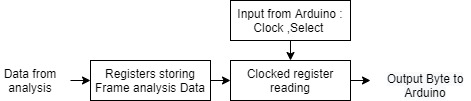
\includegraphics[width=1\linewidth, height=0.08\textheight]{ArduinoComms.jpg}
        \caption{Arduino Comms overview}
        \label{fig:ArduinoComms}
    \end{minipage}%
\end{figure}


\newpage


This left us with a final design criteria list as such :

\begin{enumerate}
\itemsep0em
  \item Detect All five balls independently. 
        \begin{enumerate}
            \itemsep-0.2em
            \item Consistently highlight pixels belonging to balls in a plain environment.
                \begin{enumerate}
                    \itemsep-0.2em
                    \item Highlight ball in multiple levels of brightness
                    \item Highlight the intended colour of ball and no others.
                    \item Eliminate (Do not highlight) the environment that is not the intended ball.
                \end{enumerate}
            \item Filter/Ignore noise data that may exist in the image.
                \begin{enumerate}
                    \itemsep-0.2em
                    \item Successfully remove any data that has been highlighted incorrectly when isolating the ball. 
                    \item Successfully avoid removing the correctly highlighted pixels of the ball.
                \end{enumerate}
            \item Accurately find minimum and maximum bounds for balls in the environment .
                \begin{enumerate}
                    \itemsep-0.2em
                    \item Ensure associated Ymin and Ymax are accurate through visual confirmation. 
                    \item Update Ymin and Ymax accordingly with each frame 
                \end{enumerate}
            \item Calculate distance to from ball to rover from image. 
                \begin{enumerate}
                    \itemsep-0.2em
                    \item Calculate the distance from rover to ball within 5\verb|%| of real distance 
                \end{enumerate}
        \end{enumerate}
  \item Detect obstructions of unknown visual data .
        \begin{enumerate}
            \itemsep-0.2em
            \item Applying filtering to reveal edges in image.
                \begin{enumerate}
                    \itemsep-0.2em
                    \item Reveal all Horizontal edges in an image through highlighting confirm visually
                    \item Extract meaningful depth data from highlighted edges. 
                \end{enumerate}
            \item Calculate the distance to edges from past and present image data.
                 \begin{enumerate}
                    \itemsep-0.2em
                    \item Reveal all Horizontal edges in an image through highlighting confirm visually
                    \item Extract meaningful depth data from highlighted edges. 
                    \item Store depth data to be outputted sent to control subsystem for analysis
                \end{enumerate}
        \end{enumerate}
  \item Relay information on detected objects to Control subsystem for further processing.
        \begin{enumerate}
            \itemsep-0.2em
            \item Instantiate a memory that can store all data of from analysis of current frame. 
            \item Relay data gathered and calculated in an agreed format to Control subsystem.
            \item Check relayed data is accurately received on the Command / Control subsystem. 
        \end{enumerate}
\end{enumerate}



\newpage


\subsubsection{Command}
The rover command module was designed to provide two main functions. Firstly, it had to provide an interface to allow the user to send commands to the rover in different formats and provide information back to the user with regard to the rovers position and sensor data. Secondly, the module had to provide drive commands to the rover based on the user input and on the vision data sent to it from the rover. 
\smallbreak
The different types of commands that we decided to allow the user to send are as follows:
\begin{enumerate}
  \item Commands in the form of a coordinate relative to the rovers current position, with the rover deciding the best route to reach the destination.
  \item Direct commands such as move forward and turn that the rover follows exactly.
  \item Commands to move to a given ball and search for it if it's position is unknown. 
\end{enumerate}
The information that would be sent back to the user can be broken down as follows:
\begin{enumerate}
  \item Provide visual indication of the position of any detected balls relative to the rover position.
  \item Provide and indication of the current charge and battery health of the rover.
  \item Provide a list of the commands the rover still has to complete.
  \item Display the current drive mode that the rover is in.
  \item Display depth data for any object in front of the rover.
\end{enumerate}
In order to allow this requirements to be filled it a map based system was decided upon, this would allow the user to easily click on a position that they desired the rover to move to whilst also displaying the current position of any balls within the same format. In order to allow for commands to be entered a textual input format would also be needed. In addition to ball detection we also decided to try and find some way of estimating the depth in front of the rover to any obstacle using the difference between two successive frames. It was unclear at the beginning of the project however if this would be possible.
\smallbreak
When calculating the actual commands to send to the rover the command module would use three different modes.
\begin{enumerate}
  \item Map mode: In this mode the rover would be sent a small movement to take it towards the target coordinate. This movement would incorporate obstacle avoidance for any balls in the rovers path.
  \item Command mode: In this mode the rover would be sent a small movement that would be a division of a command sent by the user. The rover would be continuously sent these incremental commands as it completed them until the entire user command was completed.
  \item Search mode: In this mode the rover would be searching for a given ball, if the balls position was node the same method as map mode would be used, with the ball as the target location. If the balls position was unknown a searching route would have to be implemented instead.
\end{enumerate}
It was decided that whenever the rover completed a movement sent to it from command it would send back its change in position and orientation along with any sensor data, this would allow the command module to calculate the new command to send the rover.


\subsubsection{Control}

%%%%%%%%%%%%% FUNCTIONAL DESIGN %%%%%%%%%%%%%%%%%%%%
The Control subsystem task is to provide fast and reliable data
transfer between the different subsystems. 
\medskip
This task can broken into smaller sub-tasks:
\begin{itemize}
    \item communication with the Command subsystem
    \item communication with the Drive subsystem
    \item communication with the Vision subsystem
    \item communication with the Energy subsystem
\end{itemize}

The ESP32 is what controls and manages the flow of information. It collects data from every subsystem, sends it to the server for processing and finally receives back data to reach the next destination.
\smallbreak
In particular the flow of information proceeds as follows:

\begin{figure}[hbt!]
    \centering
    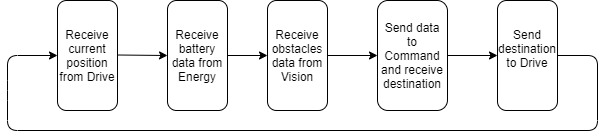
\includegraphics[scale=0.35]{esp32_flowchart.png}
    \captionsetup{justification=centering}
    \caption{High Level data flow}
\end{figure}
 
It was decided that that the Energy subsystem should not only be able to send information but also to receive it. Sending data to Energy is not shown in the diagram and happens in parallel with the main flow of information. The details are discussed in the Control Implementation section.

\paragraph{Command communication}
The Command subsystem needs to easily extract and manipulate the data sent from the Esp32. For this reason we decided to make use of JSON documents as our file format for data interchange. Communication with the Command subsystem (server) exploits WiFi connection and http requests.
%justify why you picked http
%talk about JSON objects

\paragraph{Vision communication}
The Vision subsystem needs to send large amount of processed image data to the server. For this reason the communication protocol that we picked was SPI as it's the fastest protocol that esp32 supports

\paragraph{Drive and Energy communication}
The Drive and Energy subsystems both send and receive data from the server. Since only a very small amount of data is exchanged between the esp32 and Drive or Energy, and since the esp32 supports distinct 2 UART ports, the communication protocol that we picked was UART

\begin{figure}[hbt!]
    \centering
    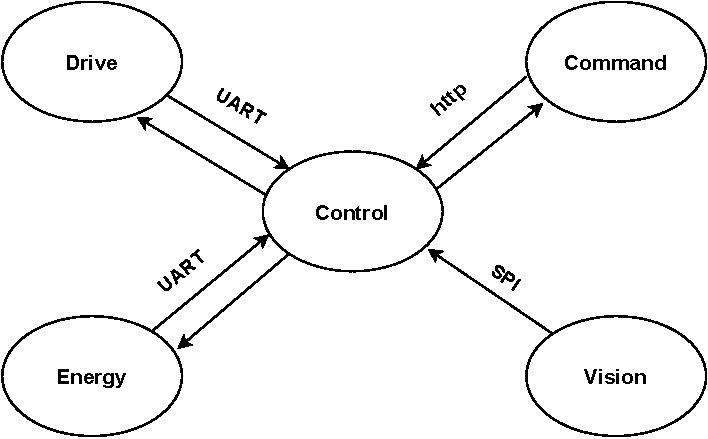
\includegraphics[scale=0.40]{esp32_comms.pdf}
    \captionsetup{justification=centering}
    \caption{communication protocols}
\end{figure}


\subsubsection{Integration}

\newpage
\subsection{Design Overview / Implementation Strategy}

\subsubsection{Drive}

\subsubsection{Energy}
\textbf{Arduino - Charge Strategy}

To get the most capacity out of a single cell, a CC/CV (Constant Current/ Constant Voltage) charge strategy was decided upon. This involves charging a cell with a steady current until the maximum voltage is reached. Both the charging current and maximum voltage are dictated by the data sheet of the cell in use (Appendix \ref{appendix:Energy}.\ref{fig:CellSpecification}). The cell is then charged using a constant voltage whereby the current slowly decreases as seen in figure \ref{fig:CCCVCharging}. This ensures that the maximum cell voltage is not surpassed while still trickle charging the cell to near maximum.
\begin{figure}[hbt]
    \centering
    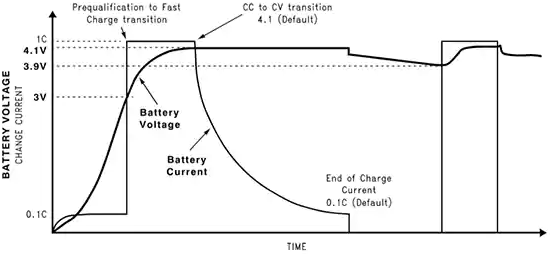
\includegraphics[scale = 0.75]{CCCV Charging.PNG}
    \caption{CC/CV Charging Example with Lithium Ion Cell \quad Source: \cite{ADigiKey}}
    \label{fig:CCCVCharging}
\end{figure}

\textbf{Arduino - SOC}

Measuring the state of charge is difficult to determine in real time due to a range of factors. This includes fluctuations in temperature and the degradation of the cell as the number of charge-discharge cycles increases. The computation power of the Arduino is also another factor to consider and therefore an Enhanced Coulomb Counting method \cite{Ng2009EnhancedBatteries} was decided upon This will work out the amount of charge going in/out of the cell and thereby the change in the SOC. Therefore, an initial value of the SOC will also be needed. Given the direct relationship between the SOC and OCV (Open Circuit Voltage), a lookup table can be extracted from early cell characterisation. This is also tightly integrated with SOH Maintenance to allow for auto calibration and integration with the passive balancing algorithm. (\ref{fig:SOCFlow}). 

\begin{figure}[hbt]
    \centering
    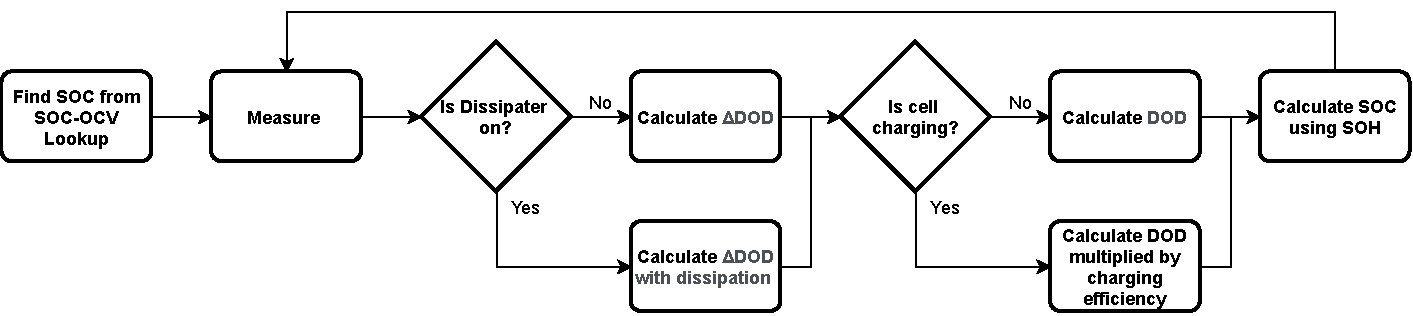
\includegraphics[width = \textwidth]{ColoumbCounting (2).pdf}
    \caption{Top level SOC finding algorithm}
    \label{fig:SOCFlow}
\end{figure}


\noindent\begin{minipage}{.32\linewidth}
\begin{equation}
    SOC = 1 - DOD
  \label{equ:SOC}
\end{equation}
\end{minipage}
\begin{minipage}{.32\linewidth}
\begin{equation}
    SOH = \frac{Q_{Discharge}^{Max}}{Q_{Rated}}
  \label{equ:SOH}
\end{equation}
\end{minipage}
\begin{minipage}{.32\linewidth}
\begin{equation}
    \eta_c = \frac{Q_{Discharge}^{Max}}{Q_{Charge}^{Max}}
  \label{equ:ChargeEfficiency}
\end{equation}
\end{minipage}

In (\ref{equ:SOC}), the state of charge can be represented as a decimal or a percentage. It is a measure of the current capacity of the cell. The state of health (\ref{equ:SOH}) is defined as the maximum discharge capacity compared to the rated capacity of the cell. It can also be represented as a percentage of the rated capacity. The charge efficiency (\ref{equ:ChargeEfficiency}) is used to create a more accurate Coulomb counting algorithm whereby the increased capacity needed during charging is accounted for as seen in figure \ref{fig:SOCFlow}.   

\noindent\begin{minipage}{.49\linewidth}
\begin{equation}
    \Delta DOD = \frac{I_{Bat}}{3600*SOH*Q_{Rated}}
  \label{equ:DeltaDOD}
\end{equation}
\end{minipage}
\begin{minipage}{.49\linewidth}
\begin{equation}
    DOD_{(k+1)} = DOD_{(k)} - \eta\Delta DOD
  \label{equ:DOD}
\end{equation}
\end{minipage}

In discrete one second intervals, $\Delta DOD$ (\ref{equ:DeltaDOD}) is seen to be the amount of amp-hours in the sampling period compared to the maximum discharge capacity which has been expanded to include the SOH. During charging, the next value of depth of discharge (\ref{equ:DOD}) decreases with an $\eta = \eta_c$. Conversely, the DOD increases during negative current (Out of cell) with $\eta=1$.

\textbf{Arduino - SOH Maintanance}

The state of health decreases as the number of charge-discharge cycles begins to accumulate. Hence it is important to track this in order to keep an accurate Coulomb Counting algorithm. This can be done by calibrating the SOH and $\eta_c$ during a full charge/discharge. Ideally this would happen after 1-2 full charge discharge cycles which would allow the coulomb count to zero itself. To prolong the life of a cell in a battery pack, an SOH maintenance strategy must be employed. This is needed to prevent a single, smaller cell, from restricting the larger cells from charging to maximum capacity. The smaller cell would then degrade at a faster rate than the others leading a lower overall battery capacity. This strategy involves developing a system to keep the various SOCs at around the same level. There are a range of balancing strategies open to us. The simplest and most effective is passive cell balancing. This involves using dedicated dissipation resistors through which the individual cells can discharge to lower their respective SOC to that of the whole battery pack. This seemed like the most obvious option given the already implemented dissipation resistors in the battery PCBs. The balancing algorithm was then idealized shown by the flowchart in figure \ref{fig:DisAlgorithm}. It should be noted that the cells should stop dissipating when they are within 3\% of its other. This is because the SOC is purely an estimation and it is needless to carry on wasting power.

\begin{figure}[hbt]
    \centering
    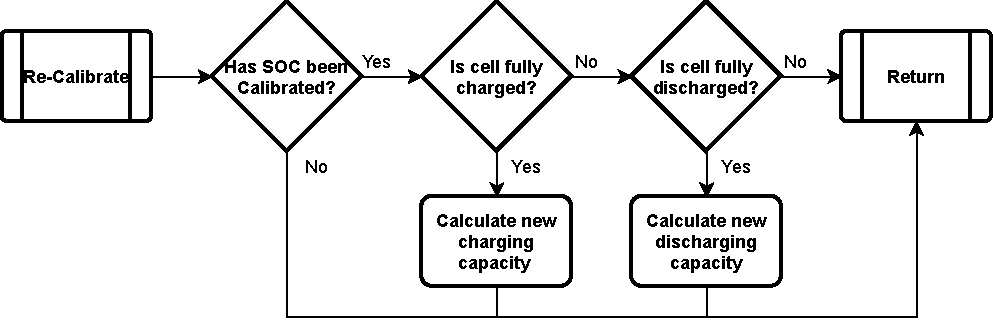
\includegraphics[scale = 0.75]{Recalibration.pdf}
    \caption{Dissipation algorithm}
    \label{fig:DisAlgorithm}
\end{figure}

\noindent\begin{minipage}{.49\linewidth}
\begin{equation}
    Q^{Max}_{{Charge}_{(k+1)}} = \frac{SOC - SOC_{Init}}{DOD_{Init}}Q^{Max}_{{Charge}_{(k)}}
    \label{equ:NewChargingCap}
\end{equation}
\end{minipage}
\begin{minipage}{.49\linewidth}
\begin{equation}
    Q^{Max}_{{Discharge}_{(k+1)}} = \frac{SOC_{Init} - SOC}{SOC_{Init}}Q^{Max}_{{Discharge}_{(k)}}
    \label{equ:NewDischargingCap}
\end{equation}
\end{minipage}

Equation \ref{equ:NewChargingCap} states that the new value of the maximum charge capacity is the ratio of the actual DOD at full capacity compared to the initial estimated DOD multiplied by the old value for the maximum capacity. Hence, if the real DOD was lower than estimated, a smaller value of charge capacity is calculated. This can then be used to find a new $\eta_c$ (\ref{equ:ChargeEfficiency}). Similarly, (\ref{equ:NewDischargingCap}) calculates a new discharge capacity by using the ratio of the actual DOD and the initial SOC. This is then applied to the previous value of the discharge capacity. Through this, a re-calibration of the SOH (\ref{equ:SOH}) and $\eta_c$ (\ref{equ:ChargeEfficiency}) can be processed.

\begin{figure}[hbt]
    \centering
    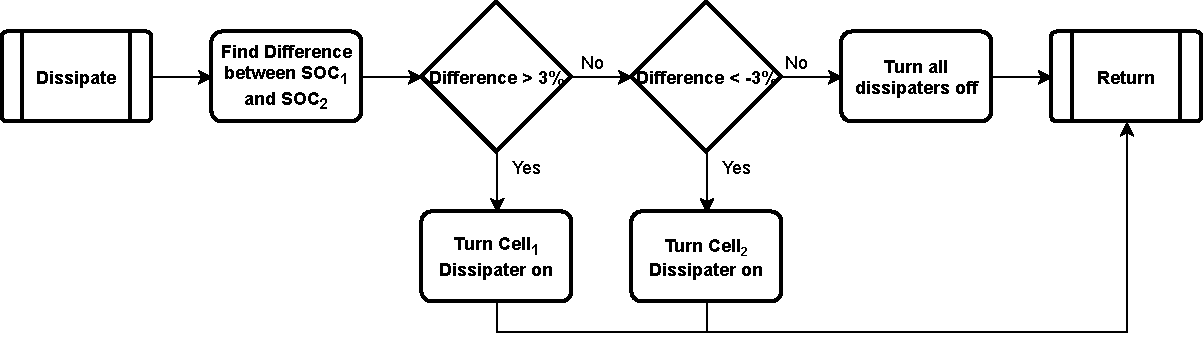
\includegraphics[scale = 0.75]{Dissipate (3).pdf}
    \caption{Dissipation algorithm}
    \label{fig:DisAlgorithm}
\end{figure}

\textbf{Arduino - PV MPPT Algorithm}

Incremental Conductance

\textbf{Arduino - Communication}

Sending/Receiving from control

\textbf{Arduino - Cell Safety}

Limits set

\textbf{Arduino - Rover Range}

Equation

\textbf{SMPS - Initial Top Level Design}

\begin{figure}[hbt]
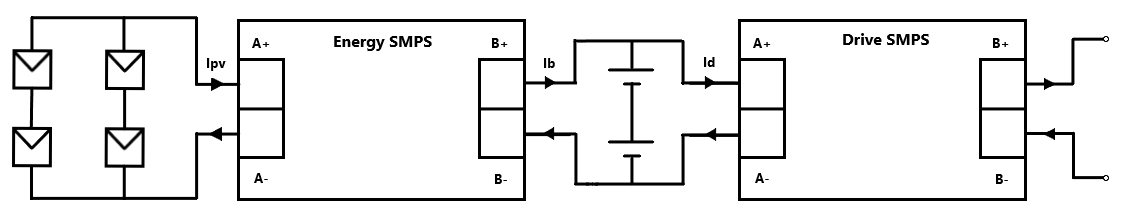
\includegraphics[width = \linewidth]{SMPS}
\centering
\caption{Preliminary design for connection to drive subsystem}
\label{fig:InitalDesign}
\end{figure}

\textbf{Battery Pack - Configuration}

Series/Potential Dividers

\textbf{PV Panels - Configuration}

2x2
\newpage
\subsubsection{Vision}

I aimed to recursively improve my design and implementation to ensure a robust and flexible subsystem that could adapt to any new criteria , tests or functionality the team agreed upon as the project progressed. This meant i would follow a development cycle illustrated below.

\begin{figure}[hbt!]
    \centering
    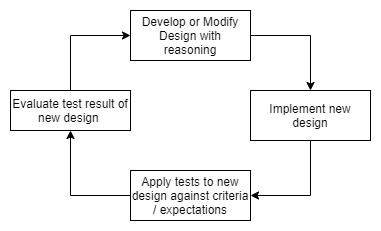
\includegraphics[scale=0.40]{FlowOfDesign.jpg}
    \captionsetup{justification=centering}
    \caption{Subsystem Development Process}
\end{figure}

I aimed to recursively improve my design and implementation to ensure a robust and flexible subsystem that could adapt to any new criteria , tests or functionality the team agreed upon as the project progressed. This meant i would follow a development cycle illustrated below.


\subsubsection{Command}

\subsubsection{Control}

\newpage

\section{Development and Implementation}

\subsection{Drive}

\subsection{Energy}

\subsection{Vision}

\textbf{Edge detection implementation:}

We use edge detection to provide more advanced data for obstacle avoidance and route planning . As well as to corroborate the hue analysis that occurs in ball detection. This provides us with a more detailed image of the environment. 
The final process implemented was this :

\begin{itemize}
    \itemsep-0.5em
    \item Store the current horizontal pixel and the previous 4 horizontal pixels in a buffer. For Gaussian analysis.
    \item Apply a 1D gaussian filter to the  pixel data in the buffer to remove noise values in the image . And output the current Gaussian filtered pixel.  
    \item From the filtered pixel data , calculate the luminance of each pixel using its RGB values. Using the formula : INSERT LUMIANNCE FORUMLA . The result of this analysis can be observed here. 
    \item Store the luminance of the current horizontal pixel and the previous 4 horizontal pixels in a buffer. 
    \item Apply a 1D Sobel to the  pixel data in the buffer to highlight edges in the image returning the Sobel value of each pixel.
    \item Using a calculated threshold , apply a white pixel value to pixels with a Sobel  value above this threshold (Implying the presence of an edge) and a black pixel value to pixels below this threshold (Implying no edge). 
\end{itemize}

This analysis produces an image with highlighted edges, of which we can now apply our distance analysis to. Allowing us to provide edge data to the Command subsystem to calculate the presence of obstacles .  

\subsection{Command}

\subsection{Control}

\section{Testing and Evaluation}
\subsection{Testing and analysis}

\subsubsection{Drive}

\subsubsection{Energy}

\subsubsection{Vision}

\subsubsection{Command}

\subsubsection{Control}

\subsubsection{Integration}

\subsection{Critical Analysis / Evaluation}

\subsubsection{Drive}

\subsubsection{Energy}

\subsubsection{Vision}

\subsubsection{Command}

\subsubsection{Control}

\subsubsection{Integration}

\section{Reflection}

\section{Essay 'Intellectual Property'}

\begin{appendices}

\section{Energy}

\setcounter{figure}{0}  %Resets the figure count
\setcounter{table}{0}   %Resets the table count



\begin{table}[htb]
    \centering
    \renewcommand{\arraystretch}{1.3}
    \begin{tabular}{||c|c|c||}
    \hline
    Specification & Value & Unit \\ [0.5ex]
    \hline \hline
    Nominal Voltage    & 3.2 & V\\
    Nominal Capacity     & 500 & mAh\\
    Minimum Voltage         & 2  & V\\
    Charging Method     & CC/CV 3.6  & V\\
    Standard Charging Current CC    & 250  & mA\\
    Continuous Discharge Current   & 500  &   mA\\
    \hline
    \end{tabular}
    \caption{Cell Specification \quad Source: Adapted from \cite{AmpsplusBattery}}
    \label{fig:CellSpecification}
\end{table}
\label{appendix:Energy}

\end{appendices}

\bibliographystyle{IEEEtranN}
\bibliography{references.bib}












\end{document}
